\section{Motivation}\label{sec:motivaiton}
Zu Beginn wurde durch eine Meinungsumfrage überprüft, ob bei Sprachassistenten mehr Datenschutz gewünscht ist. Dabei haben sich 110 Teilnehmer an der Umfragen beteiligt. Die Teilnehmer ließen sich in folgende Altersgruppen einteilen:
\begin{itemize}
	\item 0 bis 18 Jahre 
	\item 19 bis 25 Jahre
	\item 26 bis 35 Jahre
	\item 36 und älter	
\end{itemize}

\begin{figure}[h!]
	\centering
	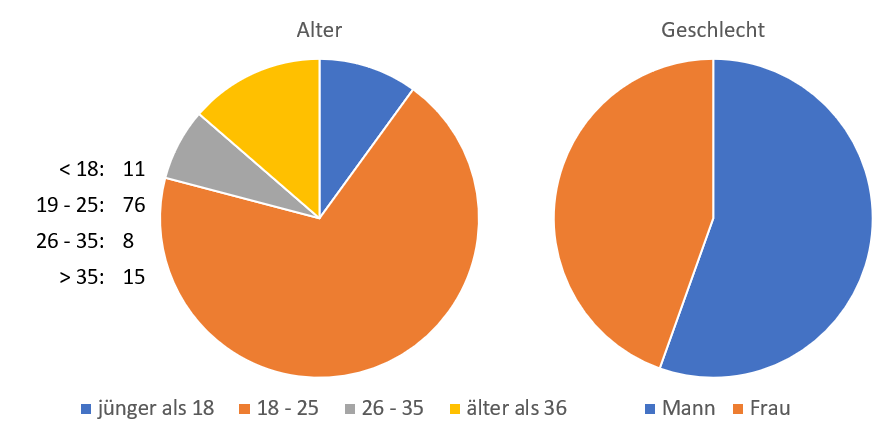
\includegraphics[width=0.7\linewidth]{Picture/umfrage_teilnehmer}
	\caption[Teilnehmer der Umfrage]{Teilnehmer der Umfrage}
	\label{fig:umfrage_teilnehmer}
\end{figure}

55,5 \% der Teilnehmer sind männlich und 45,5\% sind weiblich, wie in Abbildung \ref{fig:umfrage_teilnehmer} ersichtlich. Den Teilnehmern wurden folgende Fragen gestellt:

\begin{enumerate}	
	\item Wie oft nutzen Sie ein Sprachassistent?
	\item Wissen Sie was mit Ihren Daten passiert?
	\item Würden Sie Geld für eine hohe Datensicherheit bezahlen?
	\item Wie viel Geld würden Sie für eine hohe Datensicherheit einer Anwendung bezahlen (einmalige Zahlung)?
	\item Bei welchen Anwendungen ist Ihnen Privatsphäre besonders wichtig?	
\end{enumerate}

Bei der ersten Frage stellte sich heraus, dass 44,5\% einmal in Monat oder häufiger einen Sprachassistenten in Anspruch nehmen. In den USA wurde eine Studie von \glqq highervisibility\grqq{} durchgeführt, bei der mehr als 70\% der Teilnehmer einen Sprachassistenten einmal im Monat oder häufiger verwenden \cite{highervisibility}.
Ein direkter Vergleich der Umfrage mit der Studie aus der USA ist in Abbildung \ref{fig:umfrage_haeufigkeit} zusehen. In der Studie sind Menschen in verschiedenen Altersgruppen mit unterschiedlicher Herkunft befragt worden. Die im Rahmen dieses Artikels durchgeführte Umfrage wurde überwiegend von junge Leute beantwortet.

\begin{figure}[h!]
	\centering
	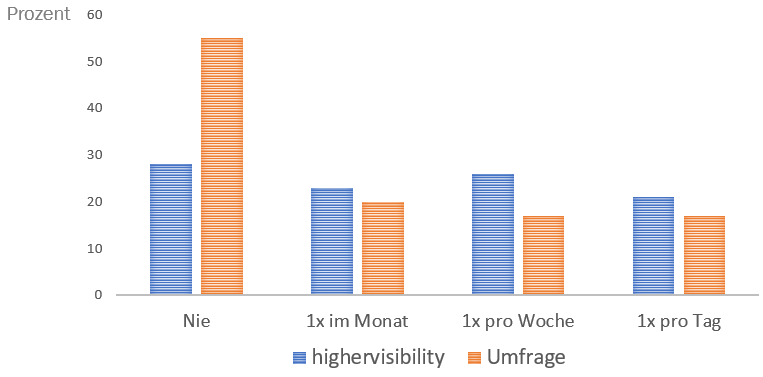
\includegraphics[width=0.7\linewidth]{Picture/umfrage_haeufigkeit}
	\caption[Nutzungshäufigkeit von Sprachassistenten]{Nutzungshäufigkeit von Sprachassistenten}
	\label{fig:umfrage_haeufigkeit}
\end{figure} 

Wie in Abbildung \ref{fig:umfrage_datenschutz} zu sehen haben 90\% der Teilnehmer angegeben, dass sie nicht wissen, was mit ihren Daten passiert. Die Zahlungsbereitschaft ist nach Altersgruppen in Abbildung \ref{fig:umfrage_geld_gruppen} visualisiert. Jeder Vierte würde dabei für eine bessere Datensicherheit Geld bezahlen und 56\% der Teilnehmer sind sich unsicher, ob diese dafür Geld bezahlen würden. Die Altersbetrachtung nach der Zahlungsbereitschaft zeigt, dass die Gruppe unter 18 Jahren weniger bereit ist, Geld zu bezahlen. Die Schnittmenge der Teilnehmern, welche Ja oder vielleicht angekreuzt haben, steigt mit zunehmendem Alter.

\begin{figure}
	\centering
	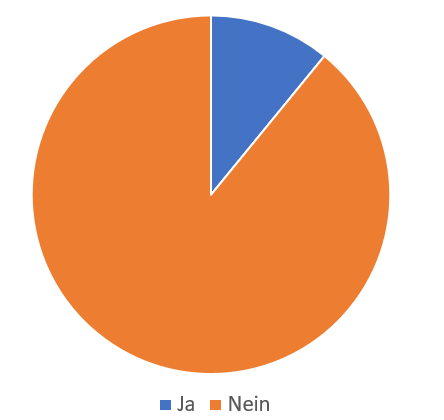
\includegraphics[width=0.5\linewidth]{Picture/umfrage_datenschutz}
	\caption[Relevanz des Datenschutzes für die Umfrageteilnehmer]{Relevanz des Datenschutzes für die Umfrageteilnehmer}
	\label{fig:umfrage_datenschutz}
\end{figure}

\begin{figure}[h!]
	\centering
	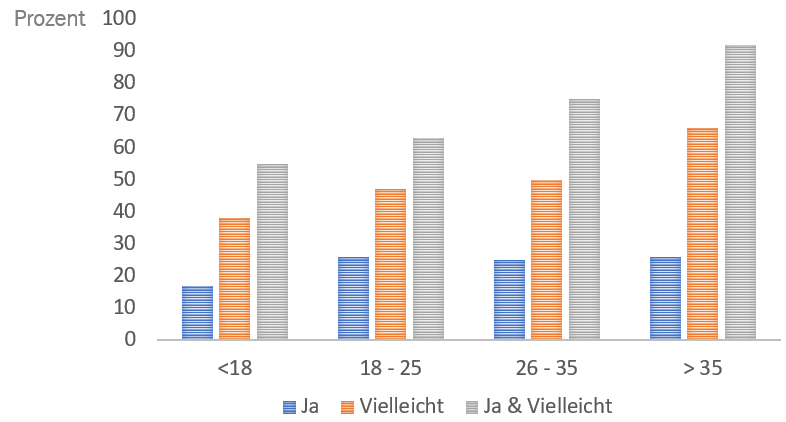
\includegraphics[width=0.7\linewidth]{Picture/umfrage_geld_gruppen}
	\caption[Zahlungsbereitschaft der Teilnehmer in verschiedenen Altersgruppen]{Zahlungsbereitschaft der Teilnehmer in verschiedenen Altersgruppen}
	\label{fig:umfrage_geld_gruppen}
\end{figure}

Der Beträge, welche die Teilnehmer für Anwendungen bezahlen würden, variiert sehr und sind in Abbildung \ref{fig:umfrage_betrag} einzusehen. Dabei sind ungefähr 15\% der Teilnehmer nicht bereit für eine Anwendung Geld zu zahlen. Der Großteil der Teilnehmer sind somit bereit für eine Anwendung Geld zu bezahlen.

\begin{figure}[h!]
	\centering
	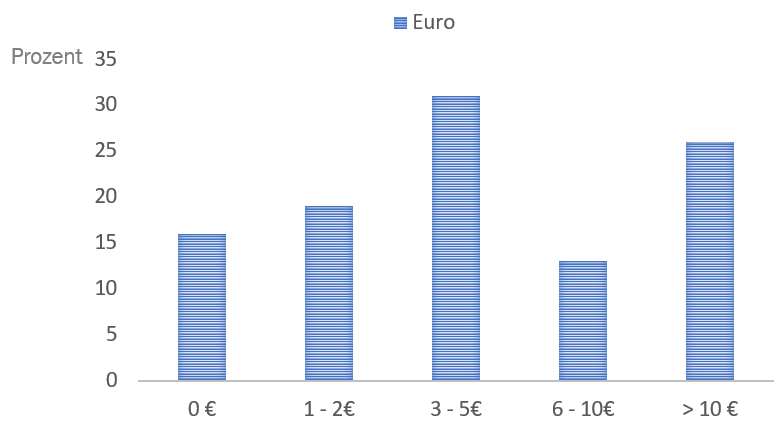
\includegraphics[width=0.7\linewidth]{Picture/umfrage_betrag}
	\caption[Zahlungsbereitschaft der Teilnehmer nach Betrag]{Zahlungsbereitschaft der Teilnehmer nach Betrag}
	\label{fig:umfrage_betrag}
\end{figure}

Wie in Abbildung \ref{fig:umfrage_anwendung} zeigt, ist den Teilnehmern die Privatsphäre im Bereich Banking, Haussteuerung, Handysteuerung, Soziale Netzwerke und Chatting besonders wichtig.

\begin{figure}[h!]
	\centering
	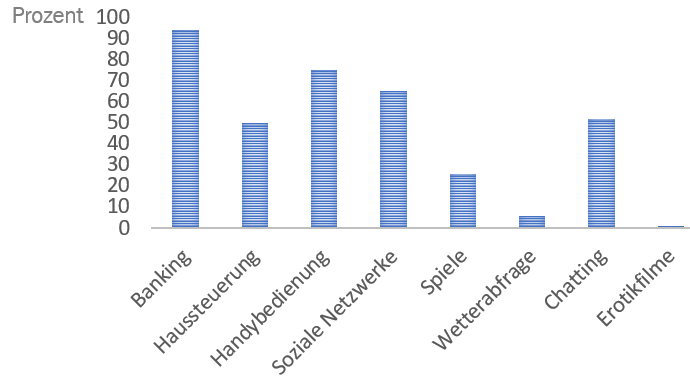
\includegraphics[width=0.7\linewidth]{Picture/umfrage_anwendung}
	\caption[Datenschutzrelevante Anwendungen der Umfrageteilnehmers]{Datenschutzrelevante Anwendungen der Umfrageteilnehmer}
	\label{fig:umfrage_anwendung}
\end{figure}

Aus der Umfragen lassen sich folgende Schlossfolgerungen ziehen:
\begin{itemize}	
	\item Personen nutzen teilweise Sprachassistenten
	\item Die Nutzer wissen nicht, was mit ihren Daten passiert
	\item Nutzer würden für eine Anwendung Geld bezahlen, wenn diese ihre Daten schützt
	\item Datenschutz ist in den Bereichen Banking, Chatting, Haussteuerung, Social Media und Handysteuerung wichtig.
\end{itemize}
